%%=============================================================================
%% LaTeX sjabloon voor bachelorproef, HoGent Bedrijf en Organisatie
%% Opleiding Toegepaste Informatica
%%=============================================================================

\documentclass[fleqn,a4paper,12pt]{book}

%%=============================================================================
%% LaTeX sjabloon voor de bachelorproef, HoGent Bedrijf en Organisatie
%% Opleiding toegepaste informatica
%%
%% Structuur en algemene vormgeving. Meestal hoef je hier niets te wijzigen.
%%
%% Vormgeving gebaseerd op "The Legrand Orange Book", version 2.0 (9/2/15)
%% door Mathias Legrand (legrand.mathias@gmail.com) met aanpassingen door
%% Vel (vel@latextemplates.com). Het oorspronkelijke template is te vinden op
%% http://www.LaTeXTemplates.com
%%
%% Aanpassingen voor HoGent toegepaste informatica: 
%%   Bert Van Vreckem <bert.vanvreckem@hogent.be>
%% Licentie: 
%%   CC BY-NC-SA 3.0 (http://creativecommons.org/licenses/by-nc-sa/3.0/)
%%=============================================================================

%%-----------------------------------------------------------------------------
%% Packages
%%-----------------------------------------------------------------------------

\usepackage[top=3cm,bottom=3cm,left=3cm,right=3cm,headsep=10pt,a4paper]{geometry} % Page margins
\usepackage[utf8]{inputenc}  % Accenten gebruiken in tekst (vb. é ipv \'e)
\usepackage{amsfonts}        % AMS math packages: extra wiskundige
\usepackage{amsmath}         %   symbolen (o.a. getallen-
\usepackage{amssymb}         %   verzamelingen N, R, Z, Q, etc.)
\usepackage[english,dutch]{babel}    % Taalinstellingen: woordsplitsingen,
                             %  commando's voor speciale karakters
                             %  ("dutch" voor NL)
\usepackage{iflang}
\usepackage{eurosym}         % Euro-symbool €
\usepackage{geometry}
\usepackage{graphicx}        % Invoegen van tekeningen
\graphicspath{{img/}}       % Specifies the directory where pictures are stored
\usepackage{tikz}            % Required for drawing custom shapes
\usepackage[pdftex,bookmarks=true]{hyperref}
                             % PDF krijgt klikbare links & verwijzingen,
                             %  inhoudstafel
\usepackage{enumitem}        % Customize lists
\setlist{nolistsep}         % Reduce spacing between list items
\usepackage{listings}        % Broncode mooi opmaken
\usepackage{multirow}        % Tekst over verschillende cellen in tabellen
\usepackage{rotating}        % Tabellen en figuren roteren

\usepackage{booktabs}        % Required for nicer horizontal rules in tables

\usepackage{xcolor}          % Required for specifying colors by name
\definecolor{maincolor}{RGB}{0,147,208} % Define the main color used for 
                             % highlighting throughout the book
                             % 0, 147, 208 = officiële kleur HoGent FBO

% Paragraph style: no indent, add space between paragraphs
\setlength{\parindent}{0em}
\setlength{\parskip}{1em}

\usepackage{etoolbox}
\usepackage{titling} % Macros for title, author, etc
\usepackage{lipsum}          % Voor vultekst (lorem ipsum)

%----------------------------------------------------------------------------------------
%	FONTS
%----------------------------------------------------------------------------------------

\usepackage{avant} % Use the Avantgarde font for headings
%\usepackage{times} % Use the Times font for headings
\usepackage{mathptmx} % Use the Adobe Times Roman as the default text font together with math symbols from the Sym­bol, Chancery and Com­puter Modern fonts

\usepackage{microtype} % Slightly tweak font spacing for aesthetics
\usepackage[utf8]{inputenc} % Required for including letters with accents
\usepackage[T1]{fontenc} % Use 8-bit encoding that has 256 glyphs

%------------------------------------------------------------------------------
%	TITLE PAGE
%------------------------------------------------------------------------------

\newcommand{\inserttitlepage}{%
\begin{titlepage}
  \newgeometry{top=2cm,bottom=1.5cm,left=1.5cm,right=1.5cm}
  \begin{center}

    \begingroup
    \rmfamily
    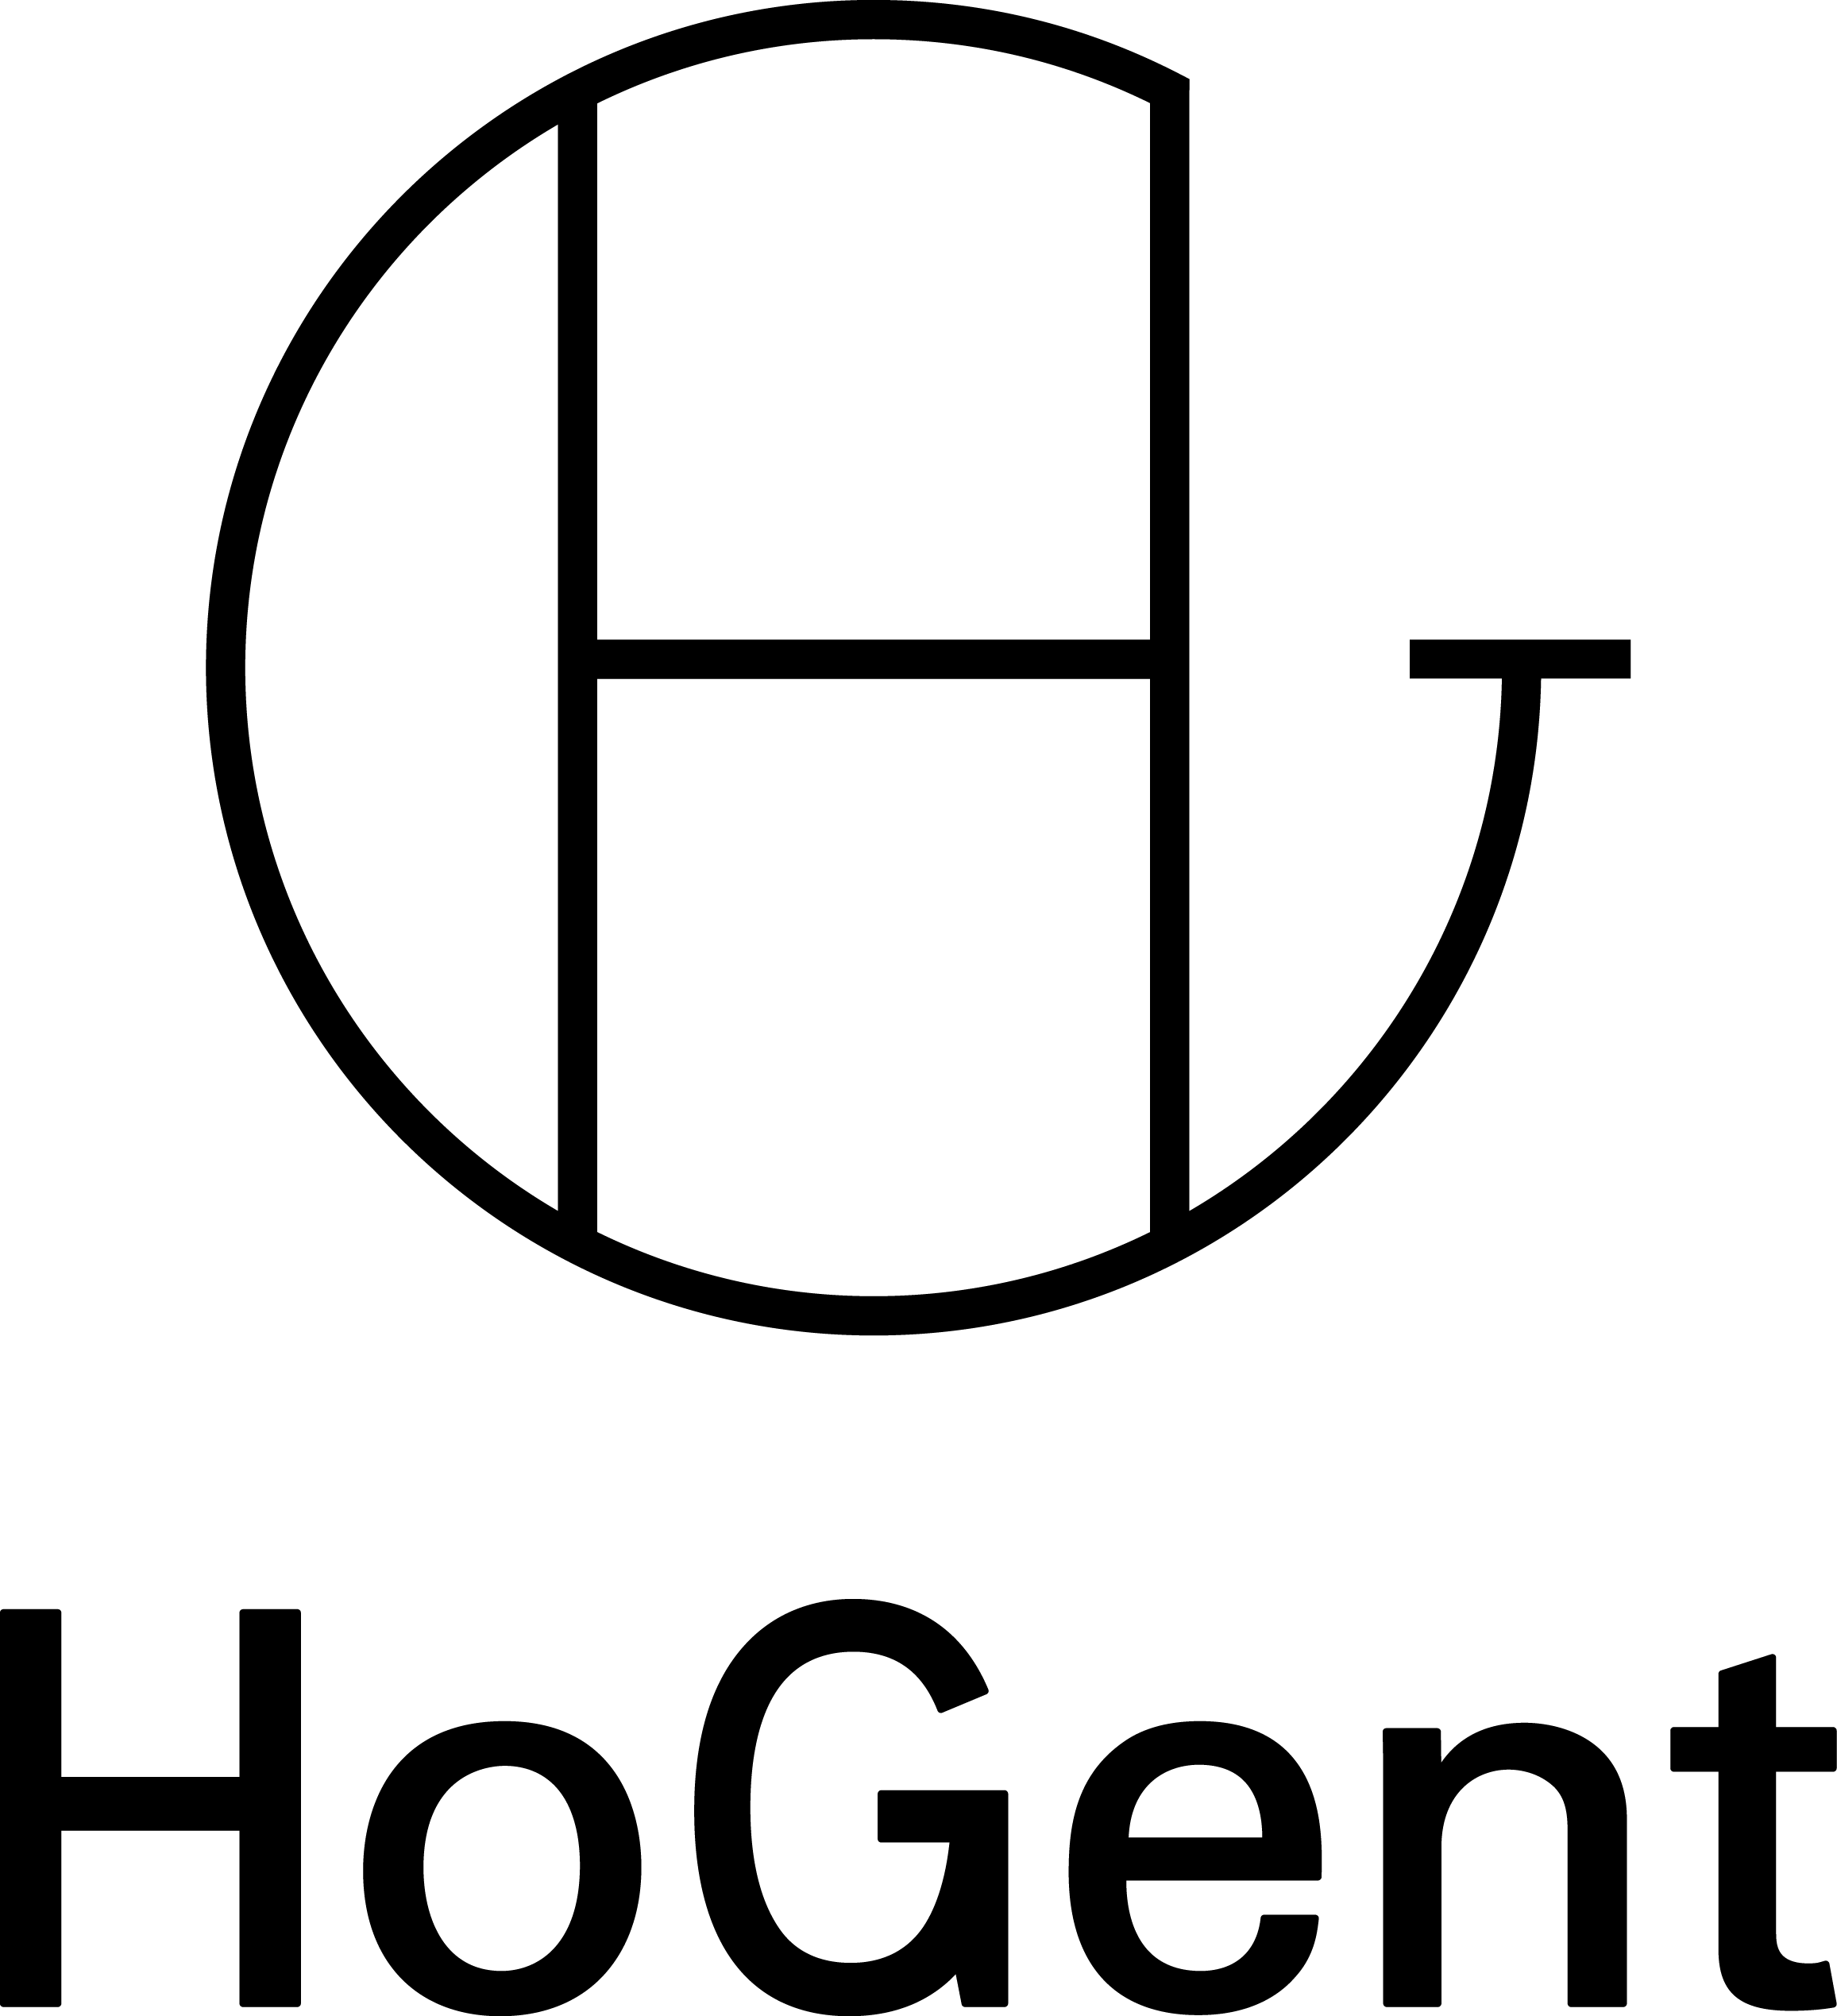
\includegraphics[width=2.5cm]{img/HG-beeldmerk-woordmerk}\\[.5cm]
    Faculteit Bedrijf en Organisatie\\[3cm]
    \titel
    \vfill
    \student\\[3.5cm]
    Scriptie voorgedragen tot het bekomen van de graad van\\professionele bachelor in de toegepaste informatica\\[2cm]
    Promotor:\\
    \promotor\\
    \ifdefempty{\copromotor}{\vspace{2.5cm}}{Co-promotor:\\\copromotor\\[2.5cm]}
    Instelling: \instelling\\[.5cm]
    Academiejaar: \academiejaar\\[.5cm]
    \ifcase \examenperiode \or Eerste \or Tweede \else Derde \fi examenperiode
    \endgroup

  \end{center}
  \restoregeometry
\end{titlepage}
  \emptypage
\begin{titlepage}
  \newgeometry{top=5.35cm,bottom=1.5cm,left=1.5cm,right=1.5cm}
  \begin{center}

    \begingroup
    \rmfamily
    \IfLanguageName{dutch}{Faculteit Bedrijf en Organisatie}{Faculty of Business and Information Management}\\[3cm]
    \titel
    \vfill
    \student\\[3.5cm]
    \IfLanguageName{dutch}{Scriptie voorgedragen tot het bekomen van de graad van\\professionele bachelor in de toegepaste informatica}{Thesis submitted in partial fulfilment of the requirements for the degree of\\professional bachelor of applied computer science}\\[2cm]
    Promotor:\\
    \promotor\\
    \ifdefempty{\copromotor}{\vspace{2.5cm}}{Co-promotor:\\\copromotor\\[2.5cm]}
    \IfLanguageName{dutch}{Instelling}{Institution}: \instelling\\[.5cm]
    \IfLanguageName{dutch}{Academiejaar}{Academic year}: \academiejaar\\[.5cm]
    \IfLanguageName{dutch}{%
    \ifcase \examenperiode \or Eerste \or Tweede \else Derde \fi examenperiode}{%
    \ifcase \examenperiode \or First \or Second \else Third \fi examination period}
    \endgroup

  \end{center}
  \restoregeometry
\end{titlepage}
}

%----------------------------------------------------------------------------------------
%	BIBLIOGRAPHY AND INDEX
%----------------------------------------------------------------------------------------

\usepackage[style=apa,backend=biber]{biblatex}
\usepackage{csquotes}
\DeclareLanguageMapping{dutch}{dutch-apa}
\addbibresource{bachproef-tin.bib} % BibTeX bibliography file
\addbibresource{../voorstel/voorstel.bib}
\defbibheading{bibempty}{}

\usepackage{calc} % For simpler calculation - used for spacing the index letter headings correctly
\usepackage{makeidx} % Required to make an index
\makeindex % Tells LaTeX to create the files required for indexing

%----------------------------------------------------------------------------------------
%	MAIN TABLE OF CONTENTS
%----------------------------------------------------------------------------------------

\usepackage{titletoc} % Required for manipulating the table of contents

\contentsmargin{0cm} % Removes the default margin

% Part text styling
\titlecontents{part}[0cm]
{\addvspace{20pt}\centering\large\bfseries}
{}
{}
{}

% Chapter text styling
\titlecontents{chapter}[1.25cm] % Indentation
{\addvspace{12pt}\large\sffamily\bfseries} % Spacing and font options for chapters
{\color{maincolor!60}\contentslabel[\Large\thecontentslabel]{1.25cm}\color{maincolor}} % Chapter number
{\color{maincolor}}
{\color{maincolor!60}\normalsize\;\titlerule*[.5pc]{.}\;\thecontentspage} % Page number

% Section text styling
\titlecontents{section}[1.25cm] % Indentation
{\addvspace{3pt}\sffamily\bfseries} % Spacing and font options for sections
{\contentslabel[\thecontentslabel]{1.25cm}} % Section number
{}
{\hfill\color{black}\thecontentspage} % Page number
[]

% Subsection text styling
\titlecontents{subsection}[1.25cm] % Indentation
{\addvspace{1pt}\sffamily\small} % Spacing and font options for subsections
{\contentslabel[\thecontentslabel]{1.25cm}} % Subsection number
{}
{\ \titlerule*[.5pc]{.}\;\thecontentspage} % Page number
[]

% List of figures
\titlecontents{figure}[0em]
{\addvspace{-5pt}\sffamily}
{\thecontentslabel\hspace*{1em}}
{}
{\ \titlerule*[.5pc]{.}\;\thecontentspage}
[]

% List of tables
\titlecontents{table}[0em]
{\addvspace{-5pt}\sffamily}
{\thecontentslabel\hspace*{1em}}
{}
{\ \titlerule*[.5pc]{.}\;\thecontentspage}
[]

%----------------------------------------------------------------------------------------
%	MINI TABLE OF CONTENTS IN PART HEADS
%----------------------------------------------------------------------------------------

% Chapter text styling
\titlecontents{lchapter}[0em] % Indenting
{\addvspace{15pt}\large\sffamily\bfseries} % Spacing and font options for chapters
{\color{maincolor}\contentslabel[\Large\thecontentslabel]{1.25cm}\color{maincolor}} % Chapter number
{}
{\color{maincolor}\normalsize\sffamily\bfseries\;\titlerule*[.5pc]{.}\;\thecontentspage} % Page number

% Section text styling
\titlecontents{lsection}[0em] % Indenting
{\sffamily\small} % Spacing and font options for sections
{\contentslabel[\thecontentslabel]{1.25cm}} % Section number
{}
{}

% Subsection text styling
\titlecontents{lsubsection}[.5em] % Indentation
{\normalfont\footnotesize\sffamily} % Font settings
{}
{}
{}

%----------------------------------------------------------------------------------------
%	PAGE HEADERS
%----------------------------------------------------------------------------------------

\usepackage{fancyhdr} % Required for header and footer configuration

\pagestyle{fancy}
\renewcommand{\chaptermark}[1]{\markboth{\sffamily\normalsize\bfseries\chaptername\ \thechapter.\ #1}{}} % Chapter text font settings
\renewcommand{\sectionmark}[1]{\markright{\sffamily\normalsize\thesection\hspace{5pt}#1}{}} % Section text font settings
\fancyhf{} \fancyhead[LE,RO]{\sffamily\normalsize\thepage} % Font setting for the page number in the header
\fancyhead[LO]{\rightmark} % Print the nearest section name on the left side of odd pages
\fancyhead[RE]{\leftmark} % Print the current chapter name on the right side of even pages
\renewcommand{\headrulewidth}{0.5pt} % Width of the rule under the header
\addtolength{\headheight}{2.5pt} % Increase the spacing around the header slightly
\renewcommand{\footrulewidth}{0pt} % Removes the rule in the footer
\fancypagestyle{plain}{\fancyhead{}\renewcommand{\headrulewidth}{0pt}} % Style for when a plain pagestyle is specified

% Removes the header from odd empty pages at the end of chapters
\makeatletter
\renewcommand{\cleardoublepage}{
\clearpage\ifodd\c@page\else
\hbox{}
\vspace*{\fill}
\thispagestyle{empty}
\newpage
\fi}

%----------------------------------------------------------------------------------------
%	THEOREM STYLES
%----------------------------------------------------------------------------------------

\usepackage{amsmath,amsfonts,amssymb,amsthm} % For math equations, theorems, symbols, etc

\newcommand{\intoo}[2]{\mathopen{]}#1\,;#2\mathclose{[}}
\newcommand{\ud}{\mathop{\mathrm{{}d}}\mathopen{}}
\newcommand{\intff}[2]{\mathopen{[}#1\,;#2\mathclose{]}}
\newtheorem{notation}{Notation}[chapter]

% Boxed/framed environments
\newtheoremstyle{maincolornumbox}% % Theorem style name
{0pt}% Space above
{0pt}% Space below
{\normalfont}% % Body font
{}% Indent amount
{\small\bf\sffamily\color{maincolor}}% % Theorem head font
{\;}% Punctuation after theorem head
{0.25em}% Space after theorem head
{\small\sffamily\color{maincolor}\thmname{#1}\nobreakspace\thmnumber{\@ifnotempty{#1}{}\@upn{#2}}% Theorem text (e.g. Theorem 2.1)
\thmnote{\nobreakspace\the\thm@notefont\sffamily\bfseries\color{black}---\nobreakspace#3.}} % Optional theorem note
\renewcommand{\qedsymbol}{$\blacksquare$}% Optional qed square

\newtheoremstyle{blacknumex}% Theorem style name
{5pt}% Space above
{5pt}% Space below
{\normalfont}% Body font
{} % Indent amount
{\small\bf\sffamily}% Theorem head font
{\;}% Punctuation after theorem head
{0.25em}% Space after theorem head
{\small\sffamily{\tiny\ensuremath{\blacksquare}}\nobreakspace\thmname{#1}\nobreakspace\thmnumber{\@ifnotempty{#1}{}\@upn{#2}}% Theorem text (e.g. Theorem 2.1)
\thmnote{\nobreakspace\the\thm@notefont\sffamily\bfseries---\nobreakspace#3.}}% Optional theorem note

\newtheoremstyle{blacknumbox} % Theorem style name
{0pt}% Space above
{0pt}% Space below
{\normalfont}% Body font
{}% Indent amount
{\small\bf\sffamily}% Theorem head font
{\;}% Punctuation after theorem head
{0.25em}% Space after theorem head
{\small\sffamily\thmname{#1}\nobreakspace\thmnumber{\@ifnotempty{#1}{}\@upn{#2}}% Theorem text (e.g. Theorem 2.1)
\thmnote{\nobreakspace\the\thm@notefont\sffamily\bfseries---\nobreakspace#3.}}% Optional theorem note

% Non-boxed/non-framed environments
\newtheoremstyle{maincolornum}% % Theorem style name
{5pt}% Space above
{5pt}% Space below
{\normalfont}% % Body font
{}% Indent amount
{\small\bf\sffamily\color{maincolor}}% % Theorem head font
{\;}% Punctuation after theorem head
{0.25em}% Space after theorem head
{\small\sffamily\color{maincolor}\thmname{#1}\nobreakspace\thmnumber{\@ifnotempty{#1}{}\@upn{#2}}% Theorem text (e.g. Theorem 2.1)
\thmnote{\nobreakspace\the\thm@notefont\sffamily\bfseries\color{black}---\nobreakspace#3.}} % Optional theorem note
\renewcommand{\qedsymbol}{$\blacksquare$}% Optional qed square
\makeatother

% Defines the theorem text style for each type of theorem to one of the three styles above
\newcounter{dummy}
\numberwithin{dummy}{section}
\theoremstyle{maincolornumbox}
\newtheorem{theoremeT}[dummy]{Theorem}
\newtheorem{problem}{Problem}[chapter]
\newtheorem{exerciseT}{Exercise}[chapter]
\theoremstyle{blacknumex}
\newtheorem{exampleT}{Example}[chapter]
\theoremstyle{blacknumbox}
\newtheorem{vocabulary}{Vocabulary}[chapter]
\newtheorem{definitionT}{Definition}[section]
\newtheorem{corollaryT}[dummy]{Corollary}
\theoremstyle{maincolornum}
\newtheorem{proposition}[dummy]{Proposition}

%----------------------------------------------------------------------------------------
%	DEFINITION OF COLORED BOXES
%----------------------------------------------------------------------------------------

\RequirePackage[framemethod=default]{mdframed} % Required for creating the theorem, definition, exercise and corollary boxes

% Theorem box
\newmdenv[skipabove=7pt,
skipbelow=7pt,
backgroundcolor=black!5,
linecolor=maincolor,
innerleftmargin=5pt,
innerrightmargin=5pt,
innertopmargin=5pt,
leftmargin=0cm,
rightmargin=0cm,
innerbottommargin=5pt]{tBox}

% Exercise box
\newmdenv[skipabove=7pt,
skipbelow=7pt,
rightline=false,
leftline=true,
topline=false,
bottomline=false,
backgroundcolor=maincolor!10,
linecolor=maincolor,
innerleftmargin=5pt,
innerrightmargin=5pt,
innertopmargin=5pt,
innerbottommargin=5pt,
leftmargin=0cm,
rightmargin=0cm,
linewidth=4pt]{eBox}

% Definition box
\newmdenv[skipabove=7pt,
skipbelow=7pt,
rightline=false,
leftline=true,
topline=false,
bottomline=false,
linecolor=maincolor,
innerleftmargin=5pt,
innerrightmargin=5pt,
innertopmargin=0pt,
leftmargin=0cm,
rightmargin=0cm,
linewidth=4pt,
innerbottommargin=0pt]{dBox}

% Corollary box
\newmdenv[skipabove=7pt,
skipbelow=7pt,
rightline=false,
leftline=true,
topline=false,
bottomline=false,
linecolor=gray,
backgroundcolor=black!5,
innerleftmargin=5pt,
innerrightmargin=5pt,
innertopmargin=5pt,
leftmargin=0cm,
rightmargin=0cm,
linewidth=4pt,
innerbottommargin=5pt]{cBox}

% Creates an environment for each type of theorem and assigns it a theorem text style from the "Theorem Styles" section above and a colored box from above
\newenvironment{theorem}{\begin{tBox}\begin{theoremeT}}{\end{theoremeT}\end{tBox}}
\newenvironment{exercise}{\begin{eBox}\begin{exerciseT}}{\hfill{\color{maincolor}\tiny\ensuremath{\blacksquare}}\end{exerciseT}\end{eBox}}
\newenvironment{definition}{\begin{dBox}\begin{definitionT}}{\end{definitionT}\end{dBox}}
\newenvironment{example}{\begin{exampleT}}{\hfill{\tiny\ensuremath{\blacksquare}}\end{exampleT}}
\newenvironment{corollary}{\begin{cBox}\begin{corollaryT}}{\end{corollaryT}\end{cBox}}

%----------------------------------------------------------------------------------------
%	REMARK ENVIRONMENT
%----------------------------------------------------------------------------------------

\newenvironment{remark}{\par\vspace{10pt}\small % Vertical white space above the remark and smaller font size
\begin{list}{}{
\leftmargin=35pt % Indentation on the left
\rightmargin=25pt}\item\ignorespaces % Indentation on the right
\makebox[-2.5pt]{\begin{tikzpicture}[overlay]
\node[draw=maincolor!60,line width=1pt,circle,fill=maincolor!25,font=\sffamily\bfseries,inner sep=2pt,outer sep=0pt] at (-15pt,0pt){\textcolor{maincolor}{R}};\end{tikzpicture}} % Orange R in a circle
\advance\baselineskip -1pt}{\end{list}\vskip5pt} % Tighter line spacing and white space after remark

%----------------------------------------------------------------------------------------
%	SECTION NUMBERING IN THE MARGIN
%----------------------------------------------------------------------------------------

\makeatletter
\renewcommand{\@seccntformat}[1]{\llap{\textcolor{maincolor}{\csname the#1\endcsname}\hspace{1em}}}
\renewcommand{\section}{\@startsection{section}{1}{\z@}
{-4ex \@plus -1ex \@minus -.4ex}
{1ex \@plus.2ex }
{\normalfont\large\sffamily\bfseries}}
\renewcommand{\subsection}{\@startsection {subsection}{2}{\z@}
{-3ex \@plus -0.1ex \@minus -.4ex}
{0.5ex \@plus.2ex }
{\normalfont\sffamily\bfseries}}
\renewcommand{\subsubsection}{\@startsection {subsubsection}{3}{\z@}
{-2ex \@plus -0.1ex \@minus -.2ex}
{.2ex \@plus.2ex }
{\normalfont\small\sffamily\bfseries}}
\renewcommand\paragraph{\@startsection{paragraph}{4}{\z@}
{-2ex \@plus-.2ex \@minus .2ex}
{.1ex}
{\normalfont\small\sffamily\bfseries}}

%----------------------------------------------------------------------------------------
%	PART HEADINGS
%----------------------------------------------------------------------------------------

% numbered part in the table of contents
\newcommand{\@mypartnumtocformat}[2]{%
\setlength\fboxsep{0pt}%
\noindent\colorbox{maincolor!20}{\strut\parbox[c][.7cm]{\ecart}{\color{maincolor!70}\Large\sffamily\bfseries\centering#1}}\hskip\esp\colorbox{maincolor!40}{\strut\parbox[c][.7cm]{\linewidth-\ecart-\esp}{\Large\sffamily\centering#2}}}%
%%%%%%%%%%%%%%%%%%%%%%%%%%%%%%%%%%
% unnumbered part in the table of contents
\newcommand{\@myparttocformat}[1]{%
\setlength\fboxsep{0pt}%
\noindent\colorbox{maincolor!40}{\strut\parbox[c][.7cm]{\linewidth}{\Large\sffamily\centering#1}}}%
%%%%%%%%%%%%%%%%%%%%%%%%%%%%%%%%%%
\newlength\esp
\setlength\esp{4pt}
\newlength\ecart
\setlength\ecart{1.2cm-\esp}
\newcommand{\thepartimage}{}%
\newcommand{\partimage}[1]{\renewcommand{\thepartimage}{#1}}%
\def\@part[#1]#2{%
\ifnum \c@secnumdepth >-2\relax%
\refstepcounter{part}%
\addcontentsline{toc}{part}{\texorpdfstring{\protect\@mypartnumtocformat{\thepart}{#1}}{\partname~\thepart\ ---\ #1}}
\else%
\addcontentsline{toc}{part}{\texorpdfstring{\protect\@myparttocformat{#1}}{#1}}%
\fi%
\startcontents%
\markboth{}{}%
{\thispagestyle{empty}%
\begin{tikzpicture}[remember picture,overlay]%
\node at (current page.north west){\begin{tikzpicture}[remember picture,overlay]%
\fill[maincolor!20](0cm,0cm) rectangle (\paperwidth,-\paperheight);
\node[anchor=north] at (4cm,-3.25cm){\color{maincolor!40}\fontsize{220}{100}\sffamily\bfseries\@Roman\c@part};
\node[anchor=south east] at (\paperwidth-1cm,-\paperheight+1cm){\parbox[t][][t]{8.5cm}{
\printcontents{l}{0}{\setcounter{tocdepth}{1}}%
}};
\node[anchor=north east] at (\paperwidth-1.5cm,-3.25cm){\parbox[t][][t]{15cm}{\strut\raggedleft\color{white}\fontsize{30}{30}\sffamily\bfseries#2}};
\end{tikzpicture}};
\end{tikzpicture}}%
\@endpart}
\def\@spart#1{%
\startcontents%
\phantomsection
{\thispagestyle{empty}%
\begin{tikzpicture}[remember picture,overlay]%
\node at (current page.north west){\begin{tikzpicture}[remember picture,overlay]%
\fill[maincolor!20](0cm,0cm) rectangle (\paperwidth,-\paperheight);
\node[anchor=north east] at (\paperwidth-1.5cm,-3.25cm){\parbox[t][][t]{15cm}{\strut\raggedleft\color{white}\fontsize{30}{30}\sffamily\bfseries#1}};
\end{tikzpicture}};
\end{tikzpicture}}
\addcontentsline{toc}{part}{\texorpdfstring{%
\setlength\fboxsep{0pt}%
\noindent\protect\colorbox{maincolor!40}{\strut\protect\parbox[c][.7cm]{\linewidth}{\Large\sffamily\protect\centering #1\quad\mbox{}}}}{#1}}%
\@endpart}
\def\@endpart{\vfil\newpage
\if@twoside
\if@openright
\null
\thispagestyle{empty}%
\newpage
\fi
\fi
\if@tempswa
\twocolumn
\fi}

%----------------------------------------------------------------------------------------
%	CHAPTER HEADINGS
%----------------------------------------------------------------------------------------

% A switch to conditionally include a picture, implemented by  Christian Hupfer
\newif\ifusechapterimage
\usechapterimagetrue
\newcommand{\thechapterimage}{}%
\newcommand{\chapterimage}[1]{\ifusechapterimage\renewcommand{\thechapterimage}{#1}\fi}%
\def\@makechapterhead#1{%
{\parindent \z@ \raggedright \normalfont
\ifnum \c@secnumdepth >\m@ne
\if@mainmatter
\begin{tikzpicture}[remember picture,overlay]
\node at (current page.north west)
{\begin{tikzpicture}[remember picture,overlay]
\node[anchor=north west,inner sep=0pt] at (0,0) {\ifusechapterimage\includegraphics[width=\paperwidth]{\thechapterimage}\fi};
\draw[anchor=west] (\Gm@lmargin,-9cm) node [line width=2pt,rounded corners=15pt,draw=maincolor,fill=white,fill opacity=0.5,inner sep=15pt]{\strut\makebox[22cm]{}};
\draw[anchor=west] (\Gm@lmargin+.3cm,-9cm) node {\huge\sffamily\bfseries\color{black}\thechapter. #1\strut};
\end{tikzpicture}};
\end{tikzpicture}
\else
\begin{tikzpicture}[remember picture,overlay]
\node at (current page.north west)
{\begin{tikzpicture}[remember picture,overlay]
\node[anchor=north west,inner sep=0pt] at (0,0) {\ifusechapterimage\includegraphics[width=\paperwidth]{\thechapterimage}\fi};
\draw[anchor=west] (\Gm@lmargin,-9cm) node [line width=2pt,rounded corners=15pt,draw=maincolor,fill=white,fill opacity=0.5,inner sep=15pt]{\strut\makebox[22cm]{}};
\draw[anchor=west] (\Gm@lmargin+.3cm,-9cm) node {\huge\sffamily\bfseries\color{black}#1\strut};
\end{tikzpicture}};
\end{tikzpicture}
\fi\fi\par\vspace*{270\p@}}}

%-------------------------------------------

\def\@makeschapterhead#1{%
\begin{tikzpicture}[remember picture,overlay]
\node at (current page.north west)
{\begin{tikzpicture}[remember picture,overlay]
\node[anchor=north west,inner sep=0pt] at (0,0) {\ifusechapterimage\includegraphics[width=\paperwidth]{\thechapterimage}\fi};
\draw[anchor=west] (\Gm@lmargin,-9cm) node [line width=2pt,rounded corners=15pt,draw=maincolor,fill=white,fill opacity=0.5,inner sep=15pt]{\strut\makebox[22cm]{}};
\draw[anchor=west] (\Gm@lmargin+.3cm,-9cm) node {\huge\sffamily\bfseries\color{black}#1\strut};
\end{tikzpicture}};
\end{tikzpicture}
\par\vspace*{270\p@}}
\makeatother

%----------------------------------------------------------------------------------------
%	HYPERLINKS IN THE DOCUMENTS
%----------------------------------------------------------------------------------------

\usepackage{hyperref}
\hypersetup{hidelinks,backref=true,pagebackref=true,hyperindex=true,colorlinks=false,breaklinks=true,urlcolor= maincolor,bookmarks=true,bookmarksopen=false,pdftitle={Title},pdfauthor={Author}}
\usepackage{bookmark}
\bookmarksetup{
open,
numbered,
addtohook={%
\ifnum\bookmarkget{level}=0 % chapter
\bookmarksetup{bold}%
\fi
\ifnum\bookmarkget{level}=-1 % part
\bookmarksetup{color=maincolor,bold}%
\fi
}
}

%----------------------------------------------------------------------------------------
%	Java source code
%----------------------------------------------------------------------------------------

% Commando voor invoegen Java-broncodebestanden (dank aan Niels Corneille)
% Gebruik:
%   \codefragment{source/MijnKlasse.java}{Uitleg bij de code}
%
% Je kan dit aanpassen aan de taal die je zelf het meeste gebruikt in je
% bachelorproef.
\newcommand{\codefragment}[2]{ \lstset{%
  language=java,
  breaklines=true,
  float=th,
  caption={#2},
  basicstyle=\scriptsize,
  frame=single,
  extendedchars=\true
}
\lstinputlisting{#1}}

% Leeg blad
\newcommand{\emptypage}{%
\newpage
\thispagestyle{empty}
\mbox{}
\newpage
}


%%---------- Documenteigenschappen --------------------------------------------
%% TODO: Vul dit aan met je eigen info:

% Je eigen naam
\newcommand{\student}{Piet Pieters}

% De naam van je promotor (lector van de opleiding)
\newcommand{\promotor}{Bert Van Vreckem}

% De naam van je co-promotor. Als je promotor ook je opdrachtgever is en je
% dus ook inhoudelijk begeleidt (en enkel dan!), mag je dit leeg laten.
\newcommand{\copromotor}{}

% Indien je bachelorproef in opdracht van/in samenwerking met een bedrijf of
% externe organisatie geschreven is, geef je hier de naam. Zoniet laat je dit
% zoals het is.
\newcommand{\instelling}{---}

% De titel van het rapport/bachelorproef
\newcommand{\titel}{Titel}

% Datum van indienen (gebruik telkens de deadline, ook al geef je eerder af)
\newcommand{\datum}{27 mei 2016}

% Academiejaar
\newcommand{\academiejaar}{2015-2016}

% Examenperiode
%  - 1e semester = 1e examenperiode => 1
%  - 2e semester = 2e examenperiode => 2
%  - tweede zit  = 3e examenperiode => 3
\newcommand{\examenperiode}{2}

%%=============================================================================
%% Inhoud document
%%=============================================================================

\begin{document}

%---------- Taalselectie ------------------------------------------------------
% Als je je bachelorproef in het Engels schrijft, haal dan onderstaande regel
% uit commentaar. Let op: de tekst op de voorkaft blijft in het Nederlands, en
% dat is ook de bedoeling!

%\selectlanguage{english}

%---------- Titelblad ---------------------------------------------------------
\inserttitlepage

%---------- Samenvatting, voorwoord -------------------------------------------
\usechapterimagefalse
%%=============================================================================
%% Voorwoord
%%=============================================================================

\chapter*{\IfLanguageName{dutch}{Woord vooraf}{Preface}}
\label{ch:voorwoord}

%% TODO:
%% Het voorwoord is het enige deel van de bachelorproef waar je vanuit je
%% eigen standpunt (``ik-vorm'') mag schrijven. Je kan hier bv. motiveren
%% waarom jij het onderwerp wil bespreken.
%% Vergeet ook niet te bedanken wie je geholpen/gesteund/... heeft

Maken als bachelorproef helemaal gedaan is.
%%=============================================================================
%% Samenvatting
%%=============================================================================

% TODO: De "abstract" of samenvatting is een kernachtige (~ 1 blz. voor een
% thesis) synthese van het document.
%
% Deze aspecten moeten zeker aan bod komen:
% - Context: waarom is dit werk belangrijk?
% - Nood: waarom moest dit onderzocht worden?
% - Taak: wat heb je precies gedaan?
% - Object: wat staat in dit document geschreven?
% - Resultaat: wat was het resultaat?
% - Conclusie: wat is/zijn de belangrijkste conclusie(s)?
% - Perspectief: blijven er nog vragen open die in de toekomst nog kunnen
%    onderzocht worden? Wat is een mogelijk vervolg voor jouw onderzoek?
%
% LET OP! Een samenvatting is GEEN voorwoord!

%%---------- Nederlandse samenvatting -----------------------------------------
%
% TODO: Als je je bachelorproef in het Engels schrijft, moet je eerst een
% Nederlandse samenvatting invoegen. Haal daarvoor onderstaande code uit
% commentaar.
% Wie zijn bachelorproef in het Nederlands schrijft, kan dit negeren, de inhoud
% wordt niet in het document ingevoegd.

\IfLanguageName{english}{%
\selectlanguage{dutch}
\chapter*{Samenvatting}
\lipsum[1-4]
\selectlanguage{english}
}{}

%%---------- Samenvatting -----------------------------------------------------
% De samenvatting in de hoofdtaal van het document

\chapter*{\IfLanguageName{dutch}{Samenvatting}{Abstract}}

Maken als bachelorproef klaar is.

\lipsum[1-4]


%---------- Inhoudstafel ------------------------------------------------------
\pagestyle{empty} % No headers
\tableofcontents % Print the table of contents itself
\cleardoublepage % Forces the first chapter to start on an odd page so it's on the right
\pagestyle{fancy} % Print headers again

%---------- Lijst figuren, afkortingen, ... -----------------------------------

% Indien gewenst kan je hier een lijst van figuren/tabellen opgeven. Geef in
% dat geval je figuren/tabellen altijd een korte beschrijving:
%
%  \caption[korte beschrijving]{uitgebreide beschrijving}

\listoffigures
\listoftables

% Als je een lijst van afkortingen of termen wil toevoegen, dan hoort die
% hier thuis. Gebruik bijvoorbeeld de ``glossaries'' package.
% https://www.sharelatex.com/learn/Glossaries

%%---------- Kern -------------------------------------------------------------

%%=============================================================================
%% Inleiding
%%=============================================================================

\chapter{\IfLanguageName{dutch}{Inleiding}{Introduction}}
\label{ch:inleiding}
In dit hoofdstuk wordt er een kort inleiding over de bachelorproef. De oorsprong van het idee en de onderzoeksvraag wordt besproken. Ook wordt er al wat basisinfo gegeven over het onderwerp.


De installatie en modificatie van software servers moet voor de gebruiker altijd makkelijker en sneller. Eens de gebruiker weet wat voor server hij wil, wil hij deze liefst zo snel mogelijk opzetten met de nodige specificaties. Of als de gebruiker een kleine aanpassing wil doen aan de server, wil hij dit zo makkelijk mogelijk aanpassen. 

Om dit zo efficiënt mogelijk te doen heb je configuration management tools nodig. Dit zijn tools die gemaakt zijn om software op servers te installeren en te beheren. De meest bekende tools zijn Chef, Puppet, Salt en Ansible. In deze bachelorproef gaat het onder andere over Ansible. 

%De inleiding moet de lezer net genoeg informatie verschaffen om het onderwerp te begrijpen en in te zien waarom de onderzoeksvraag de moeite waard is om te onderzoeken. In de inleiding ga je literatuurverwijzingen beperken, zodat de tekst vlot leesbaar blijft. Je kan de inleiding verder onderverdelen in secties als dit de tekst verduidelijkt. Zaken die aan bod kunnen komen in de inleiding~\autocite{Pollefliet2011}:

%\begin{itemize}
%  \item context, achtergrond
%  \item afbakenen van het onderwerp
 % \item verantwoording van het onderwerp, methodologie
 % \item probleemstelling
  %\item onderzoeksdoelstelling
  %\item onderzoeksvraag
  %\item \ldots
%\end{itemize}

\section{\IfLanguageName{dutch}{Context}{Problem Statement}}
\label{sec:context}

Ansible is op zich al een zeer goede configuration management tool, maar voor het bedrijf Be-Mobile nog niet goed genoeg. 

Be-Mobile is een Big Data verkeersbedrijf. Be-Mobile wil verkeer revolutioneren en de mobiliteits oplossingen voor morgen en vandaag creëren. Hun hoofdzetel ligt in Melle, bij Gent. 

Be-Mobile werkt met "Hetzner Cloud". Dit is hun cloud server provider. Met hetzner cloud heb je de optie om te verwijzen naar een cloudconfig file om je server te configureren. Het cloudconfig bestand is het configuratie  bestand van cloud-init. 

Cloud-init is net zoals een Ansible een soort van configuration management tool maar speciaal voor cloud servers. Door middel van paramaters in te vullen in dit bestand kan je jouw server configureren.
 

%Uit je probleemstelling moet duidelijk zijn dat je onderzoek een meerwaarde heeft voor een concrete doelgroep. De doelgroep moet goed gedefinieerd en afgelijnd zijn. Doelgroepen als ``bedrijven,'' ``KMO's,'' systeembeheerders, enz.~zijn nog te vaag. Als je een lijstje kan maken van de personen/organisaties die een meerwaarde zullen vinden in deze bachelorproef (dit is eigenlijk je steekproefkader), dan is dat een indicatie dat de doelgroep goed gedefinieerd is. Dit kan een enkel bedrijf zijn of zelfs één persoon (je co-promotor/opdrachtgever).

\section{\IfLanguageName{dutch}{Probleemstelling - Onderzoeksvraag}{Research question}}
\label{sec:probleemstellingonderzoeksvraag}

Het probleem is meteen heel duidelijk. Moet er worden overgestapt naar cloud-init in plaats van Ansible. In deze bachelorproef gaat dit worden onderzocht. Waar zijn Ansible en cloud-init verschillend, waar zijn ze hetzelfde en waar vullen ze mekaar aan. De echte onderzoeksvragen waar deze thesis een antwoord op hoopt te vinden is:

\begin{itemize}
    \item Is Ansible overbodig door het gebruikt van Cloud-init?
    \item Zijn Ansible en cloud-init compatibel?
    \item Op welke manier zijn ze compatibel of overbodig?
\end{itemize}



%Wees zo concreet mogelijk bij het formuleren van je onderzoeksvraag. Een onderzoeksvraag is trouwens iets waar nog niemand op dit moment een antwoord heeft (voor zover je kan nagaan). Het opzoeken van bestaande informatie (bv. ``welke tools bestaan er voor deze toepassing?'') is dus geen onderzoeksvraag. Je kan de onderzoeksvraag verder specifiëren in deelvragen. Bv.~als je onderzoek gaat over performantiemetingen, dan 

%\section{\IfLanguageName{dutch}{Onderzoeksdoelstelling}{Research objective}}
%\label{sec:onderzoeksdoelstelling}
%misschien doen
%Wat is het beoogde resultaat van je bachelorproef? Wat zijn de criteria voor succes? Beschrijf die zo concreet mogelijk. Gaat het bv. om een proof-of-concept, een prototype, een verslag met aanbevelingen, een vergelijkende studie, enz.

\section{\IfLanguageName{dutch}{Opzet van deze bachelorproef}{Structure of this bachelor thesis}}
\label{sec:opzet-bachelorproef}

% Het is gebruikelijk aan het einde van de inleiding een overzicht te
% geven van de opbouw van de rest van de tekst. Deze sectie bevat al een aanzet
% die je kan aanvullen/aanpassen in functie van je eigen tekst.

De rest van deze bachelorproef is als volgt opgebouwd:

In Hoofdstuk~\ref{ch:inleidingtotansibleencloudinit} wordt een inleding gegeven tot Ansible en cloud-init

In Hoofdstuk~\ref{ch:stand-van-zaken} wordt een overzicht gegeven van de stand van zaken binnen het onderzoeksdomein, op basis van een literatuurstudie.

In Hoofdstuk~\ref{ch:methodologie} wordt de methodologie toegelicht en worden de gebruikte onderzoekstechnieken besproken om een antwoord te kunnen formuleren op de onderzoeksvragen.

In Hoofdstuk~\ref{ch:testlokaal} worden lokale testomgevingen  opgezet doormiddel van Vagrant en Virtualbox.

In Hoofdstuk~\ref{ch:testhetzner} worden testomgevingen opgezet doormiddel van Hetzner Cloud.

In Hoofdstuk~\ref{ch:basisconf} worden er basisconfiguraties gedaan op alle servers (aanmaken users, package installeren,..)

In Hoofdstuk~\ref{ch:serverconf} worden er verschillende soorten servers(file, web, dhcp, ...) gemaakt met de testomgevingen.

In Hoofdstuk~\ref{ch:naopstarten} wordt er gekeken hoe je instellingen aanpast na het opstarten van de server.

In Hoofdstuk~\ref{ch:container} wordt gekeken de configurtie containers en clusters wordt ondersteunt.

In Hoofdstuk~\ref{ch:conclusie}, tenslotte, wordt de conclusie gegeven en een antwoord geformuleerd op de onderzoeksvragen. Daarbij wordt ook een aanzet gegeven voor toekomstig onderzoek binnen dit domein.
\chapter{\IfLanguageName{dutch}{Stand van zaken}{State of the art}}
\label{ch:stand-van-zaken}

% Tip: Begin elk hoofdstuk met een paragraaf inleiding die beschrijft hoe
% dit hoofdstuk past binnen het geheel van de bachelorproef. Geef in het
% bijzonder aan wat de link is met het vorige en volgende hoofdstuk.

% Pas na deze inleidende paragraaf komt de eerste sectiehoofding.

%Dit hoofdstuk bevat je literatuurstudie. De inhoud gaat verder op de inleiding, maar zal het onderwerp van de bachelorproef *diepgaand* uitspitten. De bedoeling is dat de lezer na lezing van dit hoofdstuk helemaal op de hoogte is van de huidige stand van zaken (state-of-the-art) in het onderzoeksdomein. Iemand die niet vertrouwd is met het onderwerp, weet nu voldoende om de rest van het verhaal te kunnen volgen, zonder dat die er nog andere informatie moet over opzoeken \autocite{Pollefliet2011}.

%Je verwijst bij elke bewering die je doet, vakterm die je introduceert, enz. naar je bronnen. In \LaTeX{} kan dat met het commando \texttt{$\backslash${textcite\{\}}} of \texttt{$\backslash${autocite\{\}}}. Als argument van het commando geef je de ``sleutel'' van een ``record'' in een bibliografische databank in het Bib\LaTeX{}-formaat (een tekstbestand). Als je expliciet naar de auteur verwijst in de zin, gebruik je \texttt{$\backslash${}textcite\{\}}.
%Soms wil je de auteur niet expliciet vernoemen, dan gebruik je \texttt{$\backslash${}autocite\{\}}. In de volgende paragraaf een voorbeeld van elk.

%\textcite{Knuth1998} schreef een van de standaardwerken over sorteer- en zoekalgoritmen. Experten zijn het erover eens dat cloud computing een interessante opportuniteit vormen, zowel voor gebruikers als voor dienstverleners op vlak van informatietechnologie~\autocite{Creeger2009}.

In dit hoofdstuk wordt de stand van zaken besproken van cloud-init en Ansible. Eerst wordt uitgelegd wat Ansible is, wat de eigenschappen zijn en hoe het precies werkt. Daarna wordt er net hetzelfde met cloud-init gedaan. Ten laatste wordt er ook een literatuurstudie uitgevoerd op gevonden van het bachelorproefvoorstel.

\section{Ansible}
Ansible is een open source IT configuration management en deployment tool. Ansible hun grote doel is om besturingssysteem configuratie en de implementatie van software allemaal onder 1 systeem. De informatie werd gevonden met behulp van het document \textit{Ansible In Depth} \autocite{ansibleid}.

Ansible staat bekend als een systeem dat makkelijk te leren is als IT administrator, ontwikkelaar of manager. Het probeert er voor te zorgen dat het makkelijk te verstaan is en makkelijk om zelf op te bouwen. Zodat nieuwe gebruikers dit makkelijk kunnen oppikken. Ze proberen uniek te zijn door dingen door val aanpassing mogelijk te geven aan gebruikers voor de expert-gebruikers. Maar toch net zo toegankelijk voor de nieuwe gebruiker.

\subsection{Architectuur}
Eén van de belangrijkste verschillen tussen Ansible en andere configuratie management tools, is zijn architectuur. Ansible gaat uit van het ``push'' model. Ook is er geen additionele software nodig om machines bruikbaar te maken voor Ansible. Het heeft geen extra gebruikers of referenties nodig om te draaien. Het gebruikt gewoon de informatie die de user meegeeft. Daarbij hoort ook dat Ansible geen administrator of sudo toegang nodig heeft. Ansible wordt standaard bestuurt door een remote computer.

Dit zorgt ervoor dat Ansible veiliger wordt. Door alleen de informatie die de gebruiker meegeeft te gebruiken. Iemand die wel toegang heeft tot de server kan maar niet tot te remote computer kan geen aanpassingen pushen.

\subsection{Playbook - Roles}
Ansible voert de automatisatie en deployment uit via playbooks. Dit zijn yaml bestanden die beschrijven hoe de automatisatie moet verlopen. 

Deze playbooks bevatten verschillende ``plays'' die de automatisatie definiëren over verschillende hosts. Deze hosts staan bekend als de inventory. Elke ``play'' bevat verschillende taken die één, verschillende of alle hosts moeten uitvoeren. Elke taak roept een Ansible module aan, een klein stukje code dat een specifieke taak uitvoert. Deze kan kunnen zeer simpel zijn, een bestand op een machine zetten of een specifieke package installeren. Maar ze kunnen ook complex zijn zoals een gehele CloudFormation opstarten in Amazon EC2.
\begin{figure}[!htb]
    \center{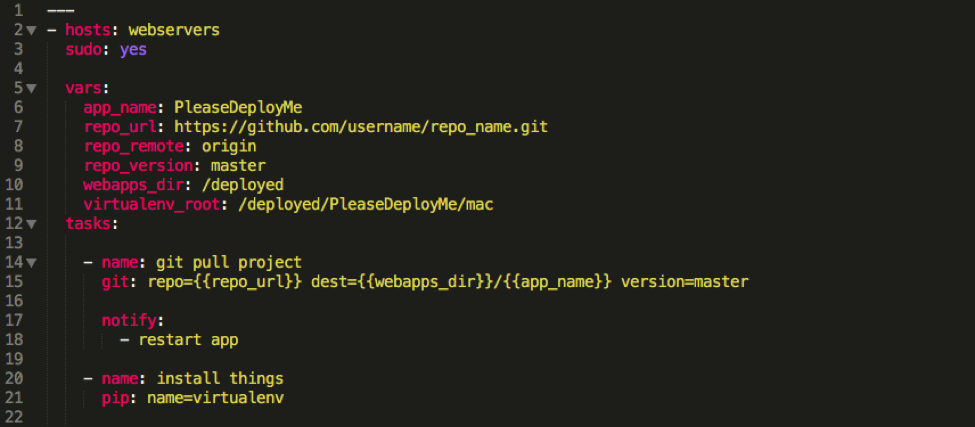
\includegraphics[width=0.9\textwidth]{img/playbookex.png}}
    \caption{Voorbeeld van een Ansible playbook.}
    \label{fig:playbook}
\end{figure}

Ansible is geschreven zodat als ze de playbook uitvoeren ook checken of deze task nog moet gedaan worden. Bijvoorbeeld als een Ansible taak is om een webserver op te starten, zal Ansible deze alleen uitvoeren als de webserver nog niet is opgestart. Dit staat bekend als idempotente. Het zorgt ervoor dat de configuratie altijd snel en efficiënt wordt uitgevoerd.

Met Ansible kunnen taken ook ingekapseld worden in een role. Dit wordt gebruikt als er een specifieke configuratie meerdere keren wordt uitgevoerd, bijvoorbeeld het opzetten van een webserver. De Ansible Galaxy site bevat veel roles die kunnen gebruikt en aangepast worden voor het gebruik in een playbook.
\begin{figure}[!htb]
    \center{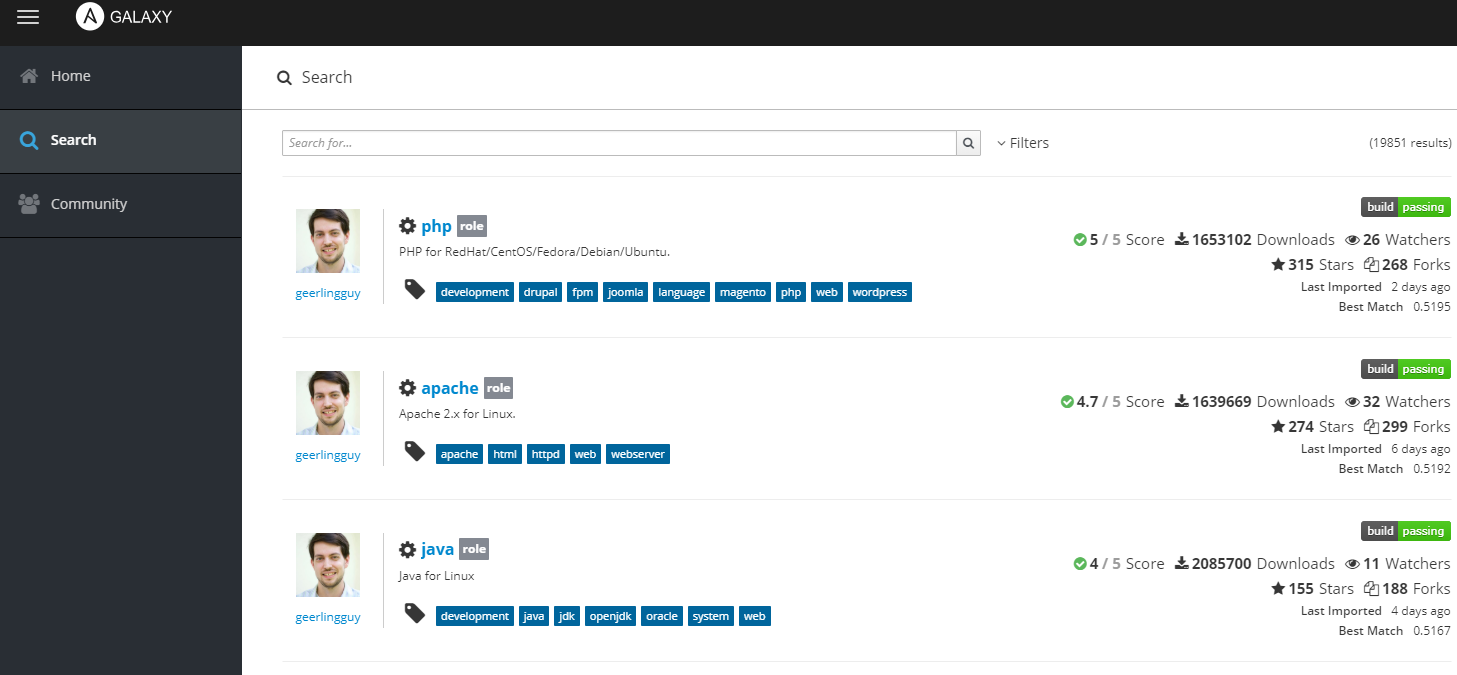
\includegraphics[width=0.9\textwidth]{img/agalaxy.png}}
    \caption{Ansible Galaxy site met lijst van roles.}
    \label{fig:agalaxy}
\end{figure}


\subsection{Omgevingen}
Ansible is even makkelijk te deployen in publieke of private cloud omgevingen, als in een lokale omgeving. Voor publieke of private cloud providers kan er gekozen worden voor: Amazon Web Services, Microsoft Azure, Rackspace,... Maar er kan ook op lokale infrastructuren gewerkt worden door middel van virtuele machines. Tools die hiervoor worden gebruikt zijn: VirtualBox, VMWare,...

\section{Cloud-Init}
Net als Ansible is cloud-init ook een soort van configuration manager en deployment tool. Het is geschreven in python. Cloud-init zorgt  voor de customisaties tijdens het opstarten van de cloud of virtuele instanties. Deze service gebeurt heel vroeg in het boot proces. De instantie zoekt naar de \textit{user data} (het cloud-init script) van de gebruiker en voert deze uit. De naam zegt het al zelf, maar cloud-init is een tool die meer wordt gebruikt door cloud instanties. Bijna alle cloud-providers hebben een functie waardoor er een cloud-init script kan meegeven worden. 

Veel van de punten die hier verder worden besproken zijn gevonden in de presentatie van \autocite{cloudred}.

\subsection{Modules}
Cloud-init heeft 6 hoofdpijlers waar het modules voor heeft, namelijk: schijf configuratie, commando's uitvoeren, gebruikers en groepen creeeren, beheren van packages, content bestanden schrijven en bootstrappen van Chef en/of Puppet. Er zijn nog andere modules maar dit zijn de 6 hoofdpijlers van cloud-init en daarbij de meeste gebruikte modules. Er kunnen ook zelf modules toevoegd worden door deze in Python te schrijven. Met behulp van de documentatie van \textcite{clouddocs} wordt er per pijler uitleg gegeven. 

\subsubsection{Schijf configuratie}
Er is 1 module die wordt gebruikt voor de schijf configuratie, namelijk \textbf{Disk Setup}. Via deze module kunnen er simpele paritities en bestandsystemen worden geconfigureerd. Via de \textit{device\_aliases} richtlijnen kunnen er aliassen worden gemaakt voor de de block devices. Zodat er makkelijker naar deze kan worden verwezen. Via de \textit{disk\_setup} richtlijn wordt de partitie configuratie gedaan. De \textit{table\_type} richtlijn wordt gebruikt om de partitie tabel mee te gegeven. Ten laatste is er ook de \textit{fs\_setup} richtlijn deze wordt gebruikt om de systeembestand configuratie te doen.

\subsubsection{Commando's uitvoeren}
Voor het uitvoeren van commando's zijn er 2 modules: \textbf{Runcmd} en \textbf{Bootcmd}. Beide bevatten maar 1 richtlijn namelijk \textit{runcmd} en \textit{bootcmd}. Bij \textit{runcmd} worden de command's die worden meegegeven elke keer uitgevoerd als het script wordt gedraaid. Bij \textit{bootcmd} enkel alleen als de instantie wordt opgestart. Ook worden de commando's bij \textit{bootcmd} veel vroeger in het bootproces uitgevoerd.

\subsubsection{Gebruikers en groepen}
Ook voor Gebruikers en groepen is er slechts 1 module: \textbf{Users and Groups}. Groepen kunnen worden toegevoegd door deze aan de richtlijn \textit{groups} toe te voegen samen eventuele configuratie per groep. Gebruikers kunnen dan weer toegevoegd worden door deze aan de richtlijn \textit{users} toe te voegen. Ook bij de gebruikers kan er nog extra configuratie gedaan worden per gebruiker.

\subsubsection{Packages}
Voor het beheren en configueren van packages zijn er verschillende modules: \textbf{Apt Configure}, \textbf{Apt Pipelining}, \textbf{Package Update Upgrade Install}, \textbf{Snap}, \textbf{Snappy} en \textbf{Yum Add Repo}. Er kunnen packages geïnstalleerd en geconfigureerd worden via Yum en Apt. Meestal ondersteund een besturingsysteem Yum of Apt. Voor installatie van een package moeten deze plaatsen bij de richtlijn \textit{packages}. Cloud-init weet zelf of het met yum of apt wordt gedaan. De configuratie en het toevoegen van package repo's gebeurt via Apt Configure, Apt Pipelinig en Yum Add Repo. Ook ondersteunt cloud-init de installatie van snap packages. Dit zijn gecontaineriseerde packages. Via Snappy kan deze geconfigureerd worden.

\subsubsection{Content bestanden}
Voor het aanmaken van bestanden is er de module \textbf{Write Files}. In de richtlijn \textit{write\_files} word de gecodeerde inhoud van het bestand gezet met het pad.

\subsubsection{Chef - Puppet}
Ook zijn er 2 modules die Chef en Puppet installeren, configureren en starten. Deze modules zijn logischer wijs \textbf{Chef} en \textbf{Puppet}. Voor Puppet wordt de richtlijn \textit{puppet} meegegeven. Daaronder worden alle configuraties geplaatst. Chef werkt op dezelfde manier.

\subsection{User Data - Cloud config}
Zoals Ansible zijn playbook heeft, heeft cloud-init zijn user data. Ook heeft cloud-init de meta-data, maar deze wordt meegegeven door het cloud platform zelf. Dit zijn bijvoorbeeld de server naam en het server id. De 2 bekendste methodes om user data mee te geven zijn User-Data Script en Cloud Config Data. 
\subsubsection{User-Data Script}
Het User-Data script een linux script dat de server overloopt voor dat hij opstart. Het moet alijd beginnen met \textit{!\#} of \textit{Content-Type: text/x-shellscript}. Als er echt wordt gebruikt gemaakt van cloud-init wordt deze methode niet gebruikt. De modules kun je via zo een script bijvoorbeeld niet aanroepen. Dit is eerder voor gebruikers die al een script hebben. In plaats van dit om te zetten naar Cloud Config Data, kunnen ze dat dan script gebruiken.
\begin{figure}[!htb]
	\center{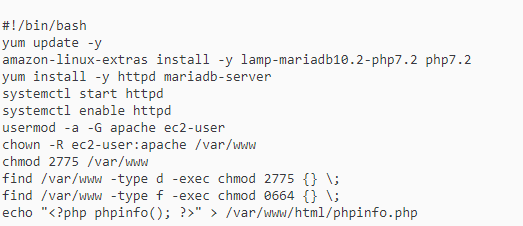
\includegraphics[width=0.9\textwidth]{img/userdatascript.png}}
	\caption{Voorbeeld user-data script.}
	\label{fig:udatascript}
\end{figure}

\subsubsection{Cloud Config Data}
De meest gebruikte methode is Cloud Config Data. Dit is een yaml bestand met de configuratie van de server in. Een Cloud Config bestand begint altijd met \textit{\#cloud-config}. In het bestand worden de modules opgelijst die worden gebruikt en daaronder dan hun configuraties. Dit bestand is veel overzichtelijker dan een script om later aan te passen of om te beheren. Ook heeft het wat gelijkenissen met het playbook van Ansible, doordat dit beide yaml bestanden zijn.
\begin{figure}[!htb]
	\center{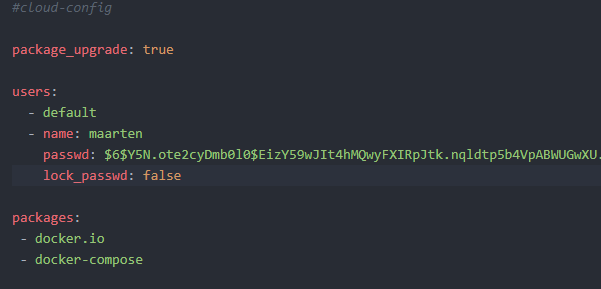
\includegraphics[width=0.9\textwidth]{img/cloudconfig.png}}
	\caption{Voorbeeld Cloud Config Data.}
	\label{fig:udatascript}
\end{figure}

\section{Studie 1}


%%=============================================================================
%% Methodologie
%%=============================================================================

\chapter{\IfLanguageName{dutch}{Methodologie}{Methodology}}
\label{ch:methodologie}

%% TODO: Hoe ben je te werk gegaan? Verdeel je onderzoek in grote fasen, en
%% licht in elke fase toe welke stappen je gevolgd hebt. Verantwoord waarom je
%% op deze manier te werk gegaan bent. Je moet kunnen aantonen dat je de best
%% mogelijke manier toegepast hebt om een antwoord te vinden op de
%% onderzoeksvraag.
In dit hoofdstuk wordt besproken welke methodes er gehanteerd zijn om de resultaten te bekomen. Dit hoofdstuk is onderverdeeld in 2 delen. Ten eerste wordt er info gegeven over de 2 testomgevingen. Ten tweede wordt er besproken welke testcriteria er gekozen zijn en waarom. In deze bachelorproef wordt er vooral focus gelegd op het de praktijk, het is een praktische onderzoek.

\section{Testomgevingen}
Voor het onderzoek moeten er verschillende testomgevingen worden opgesteld, om alles in te testen. Er is een lokale virtueel  omgeving en een omgeving op cloud servers. Er is gekozen voor deze twee omgevingen omdat dit de 2 meest voorkomende omgevingen zijn in de praktijk bij server management tools. 

Ansible is al een tool die gebruikt wordt voor virtuele omgevingen door gebruikers thuis, maar ook in grote cloud omgevingen voor bedrijven. Het zou dus niet correct zijn om het alleen lokaal te testen of alleen op de cloud. 

Voor het onderzoek is dit ook interessant want er is veel meer kans op verschillende resultaten. Die kunnen dan met elkaar worden vergeleken en dan kan er worden bekeken wat de oorzaak hiervan is. Dit geeft ook een mogelijkheid om het onderzoek in de toekomst verder te onderzoeken. Waarom bijvoorbeeld Ansible beter is lokaal zonder cloud-init dan met (dit is een hypothetische stelling).

\newpage
Per omgeving is er hieronder wat meer informatie te vinden. Over het opzetten van de omgevingen zijn voor beide aparte hoofdstukken aan toegewijd, namelijk: Hoofdstuk \ref*{ch:testlokaal} en Hoofdstuk \ref*{ch:testhetzner}.

\subsection{Lokaal}
Voor de lokale omgeving zal er worden gewerkt met 2 technologieën, namelijk: VirtualBox en vagrant. 

VirtualBox is een programma waarmee je virtuele machines kunt aanmaken en beheren. Hiermee worden de servers lokaal aangemaakt. 

Het tweede programma dat wordt gebruikt is vagrant. Vagrant is een command tool die die servers configureerd. In de actieve directory wordt het commando \textit{vagrant init} gedaan, dan staat er een \textit{vagrantfile}. Dit is het bestand dat kan worden geconfigureerd naargelang de wens van de gebruiker. Daarna wordt het commando \textit{vagrant up} gedaan. Dit start de server op. De server wordt opgestart met behulp van een tool die virtuele machines beheert en aanmaakt. In dit geval dus VirtualBox.
\begin{figure}[!htb]
	\center{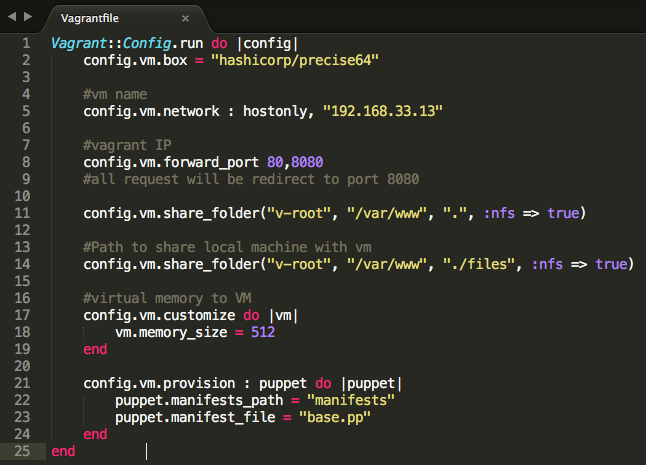
\includegraphics[width=0.9\textwidth]{img/vagrantexamp.png}}
	\caption{Voorbeeld van een vagrantfile.}
	\label{fig:vagrantexamp}
\end{figure}

\newpage
\subsubsection{Laptop}
Deze testomgeving wordt opgezet op de laptop: \textbf{Asus X750L}. Asus bracht deze laptop eind 2013 op de markt. De laptop is aangekocht in augustus 2014, en is bij het uitvoeren van het onderzoek bijna 5 jaar oud. Bijna alle specificaties zijn hetzelfde toen hij werd aangekocht. Alleen is de harde schijf vervangen van een HDD van 500 gigabyte naar een SSD van 500 gigabyte. Deze vervanging werd begin 2019 gedaan en bij het uit voeren van het onderzoek is dat 2-3 maand geleden. Hieronder is een  uitgebreide tabel met specificaties van de laptop. De data is verkregen door: \autocite{asuslaptop}.

\begin{table}
	\centering
	\begin{tabular}{c l}
		\hline
		\multicolumn{2}{c}{\textbf{Specificaties}} \\
		\hline
		Fabrikant & Asus \\
		\hline
		Model & ASUS x750L \\
		\hline		
        Besturingssysteem & Windows 10\\
        \hline
		CPU & Intel Core i7 4500U @ 2.4 GHz  \\
		\hline
		Geheugen & 8GB DDR3 @ 1600MHz \\
		\hline
		GPU & Nvidia GeForce GT 740M \\
		\hline
		Interne schijven & Crucial MX500 (500 GB) \\
		\hline
	\end{tabular}
	\caption{Specificaties van de laptop.}
	\label{tab:specs_desktop }
\end{table}

\begin{figure}[!htb]
	\center{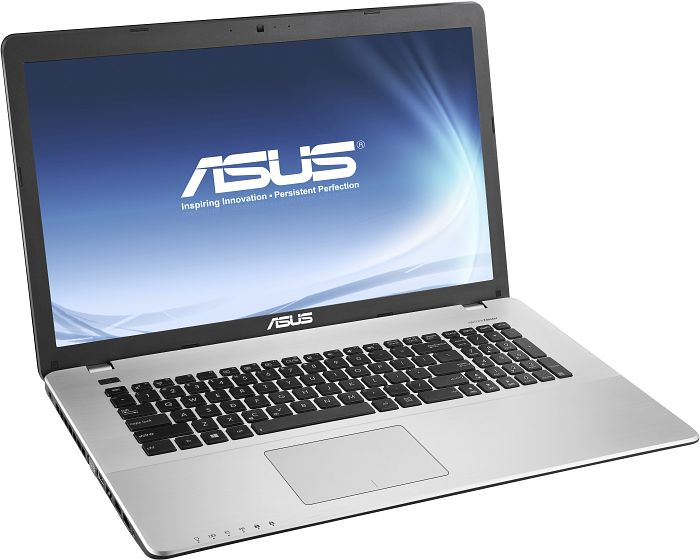
\includegraphics[width=0.4\textwidth]{img/testpcasus.jpg}}
	\caption{Foto van de laptop.}
	\label{fig:asustest}
\end{figure}

\subsection{Cloud}
Voor de cloud omgeving wordt er Hetzner Cloud gebruikt. In de inleiding is het bedrijf Be-Mobile al vernoemd en werd ook al gezegd dat zijn één van de redenen van het onderzoek zijn. Via hun is er toegang verkregen op een Hetzner Cloud omgeving om in te testen. 

Hetzner is een Duits bedrijf dat gespecialiseerd is in het hosten van servers. Hun datacenters liggen in Nuremberg (Duitsland), Falksenstein (Duitsland) en Helsinki (Finland). 

Via de commandline tool werden de server aangemaakt. Ook wordt er een SSH sleutel voorzien zodat er toegang is tot de aangemaakte servers. Info van hetzner werd gevonden dankzij de site van \autocite{hetzner}.


\section{Testcriteria}
Het volgende dat wordt besproken is de keuze van de testcriteria die werd gekozen in hoofdstukken~\ref{ch:basisconf},~\ref{ch:serverconf},~\ref{ch:naopstarten} en~\ref{ch:container}. 

In Hoofdstuk \ref*{ch:basisconf} worden basis configuraties op de server uit gevoerd. Dit om te bekijken wat de beste optie is om te kiezen als er gewoon wat kleine basis configuraties worden veranderd. Dit kan gebruikers aanmaken zijn, maar ook: commando's uitvoeren, mappen aanmaken. 

In Hoofdstuk \ref*{ch:serverconf} worden verschillende servers geïnstalleerd. Zo wordt er bekeken of het installeren en configureren van servers een ander resultaat heeft dan basis configuraties. Ook om te bekijken of er verschillen zijn per server.

In Hoofdstuk \ref*{ch:naopstarten} gaat er worden gekeken met welke optie je de server best aanpast na het opstarten. Als de server al opgestart is maar er wordt een klein dingetje verandert in het script. Welke optie is dan het best om snel deze verandering door te voeren.

Ten laatste wordt er in Hoofdstuk \ref*{ch:container} gekeken naar de configuratie van containers en clusters. Bijna elk bedrijf gebruikt containers en clusters voor hun netwerk. Het is dus logisch om te bekijken wat hier de resultaten zijn. Misschien zijn deze wel helemaal anders dan de resultaten van hiervoor.

\glossary{test}
%% Basis Configuratie, sever inst en conf, instellingen aanpassen na opstarten en container/cluster.



% Voeg hier je eigen hoofdstukken toe die de ``corpus'' van je bachelorproef
% vormen. De structuur en titels hangen af van je eigen onderzoek. Je kan bv.
% elke fase in je onderzoek in een apart hoofdstuk bespreken.

%\input{...}
%\input{...}
%...

%%=============================================================================
%% Conclusie
%%=============================================================================

\chapter{Conclusie}
\label{ch:conclusie}

% TODO: Trek een duidelijke conclusie, in de vorm van een antwoord op de
% onderzoeksvra(a)g(en). Wat was jouw bijdrage aan het onderzoeksdomein en
% hoe biedt dit meerwaarde aan het vakgebied/doelgroep? 
% Reflecteer kritisch over het resultaat. In Engelse teksten wordt deze sectie
% ``Discussion'' genoemd. Had je deze uitkomst verwacht? Zijn er zaken die nog
% niet duidelijk zijn?
% Heeft het onderzoek geleid tot nieuwe vragen die uitnodigen tot verder 
%onderzoek?

Doorheen de bachelorproef werd er gezocht naar een antwoord op de vragen. Kunnen Ansible en cloud-init samen functioneren, zo ja hoe ? Maakt cloud-init Ansible overbodig? Na een onderzoek kan er antwoord gegeven worden op die vragen. 

Het resultaat wordt hierna vergeleken met de verwachte resultaten. 

Ten laatste wordt er besproken hoe dit onderzoek kan worden uitgebreid in de toekomst. Zijn er bijkomende vragen ontstaan?

\section{Antwoord op onderzoeksvragen}
Maakt cloud-init Ansible overbodig? Nee, eigenlijk niet. In de hoofdstukken \ref{ch:serverconf} en \ref{ch:container} werd gezien dat cloud-init, voor de meer geavanceerde configuratie, toch niet de juiste oplossing is. Als er servers moesten geconfigureerd worden met meerdere rules, schoot cloud-init nog te kort. De enige module waarin in kon gewerkt hiervoor was \textit{runcmd}. Ook werd in hoofdstuk \ref{ch:naopstarten} gezien dat cloud-init geen optie heeft om wijzigingen door te voeren en het script een tweede keer te draaien. Alleszins niet in de setup die hier wordt gebruikt. Al kan cloud-init wel voor bepaalde dingen gebruikt worden. In hoofdstuk \ref{ch:basisconf} werd gezien dat voor basisconfiguraties cloud-init misschien wel beter is dan Ansible. Cloud-init maakt Ansible dus zeker niet overbodig. Hiervoor zijn de modules te gelimiteerd. Maar als er een omgeving moet worden opgezet met juist basis configuraties, is het misschien aangeraden om cloud-init hiervoor te gebruiken.

\newpage
Kunnen Ansible en cloud-init samen functioneren? Ja, dit kunnen ze zeker, maar of dit moet worden gedaan hangt af van de situatie. Het samenwerken van cloud-init zou eerder nuttig zijn voor als de server wordt aangemaakt, er meteen configuratie willen meegegeven worden. Als dit niet het geval is, is een samenwerking niet aan te raden. Ook is een samenwerking alleen van nut als de configuraties die worden gedaan meer zijn dan de basis. In hoofdstuk \ref{ch:basisconf} werd gezien dat cloud-init de basis configuraties nog alleen kan doen zonder de hulp van Ansible.

Hoe kunnen ze samen functioneren? In praktijk lijkt het best om deze samen te gebruiken met elk zijn bepaalde functies. Cloud-init is in deze setup zeer goed als initieel script, doordat dit zo makkelijk kan worden meegegeven. In dit script kunnen eerste basis configuraties worden gedaan. Hierna wordt het Ansible playbook aangeroepen met de meer geavanceerde functies.

Als er een pure vergelijking wordt gedaan tussen de beide tools, is Ansible toch de winnaar. Ansible heeft, zoals hier al meerdere keren is aangehaald, veel meer functionaliteiten dan cloud-init. Ook heeft Ansible een veel duidelijkere output (Figuur \ref{fig:outputs}). Bij cloud-init wordt veel info getoond als het script loopt, dit kan wat overweldigend zijn. Terwijl bij Ansible alles mooi is opgelijst in de verschillende taken. Ook is het hierdoor veel makkelijker om eventuele fouten uit een script te halen.
\begin{figure}[!htb]
    \centering
    {{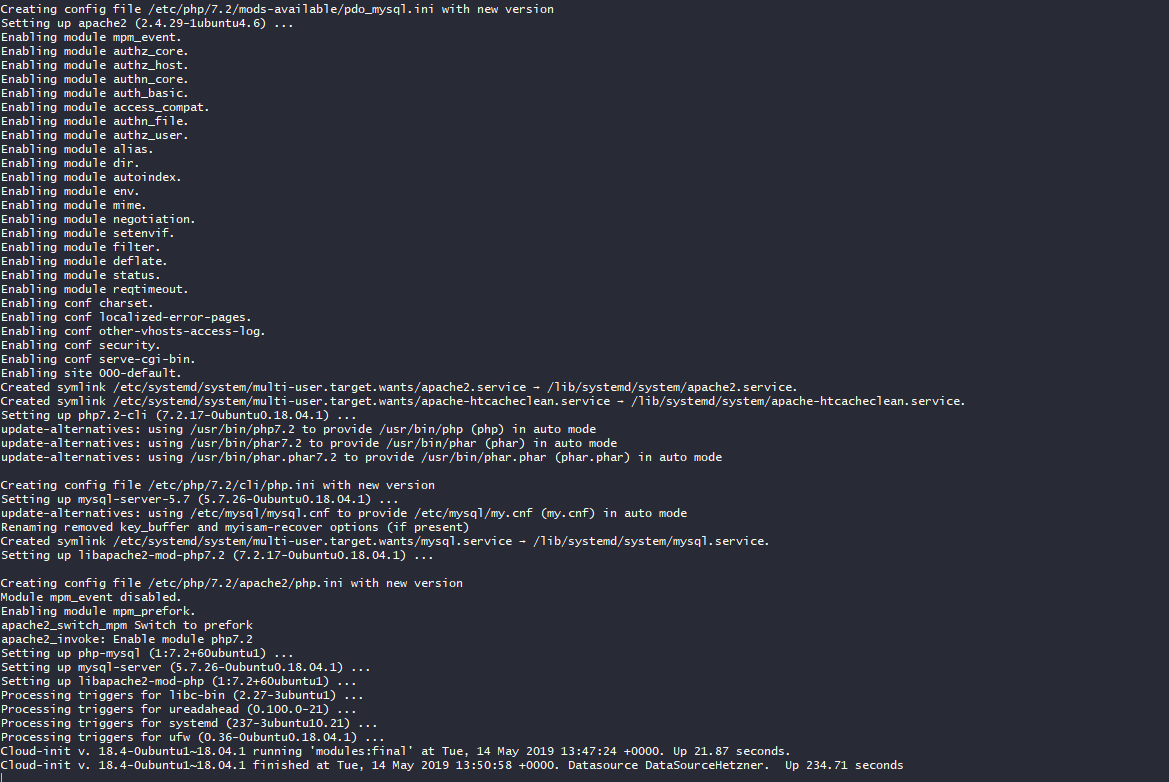
\includegraphics[width=0.45\textwidth]{img/cloudoutput.png} }}%
    \qquad
    {{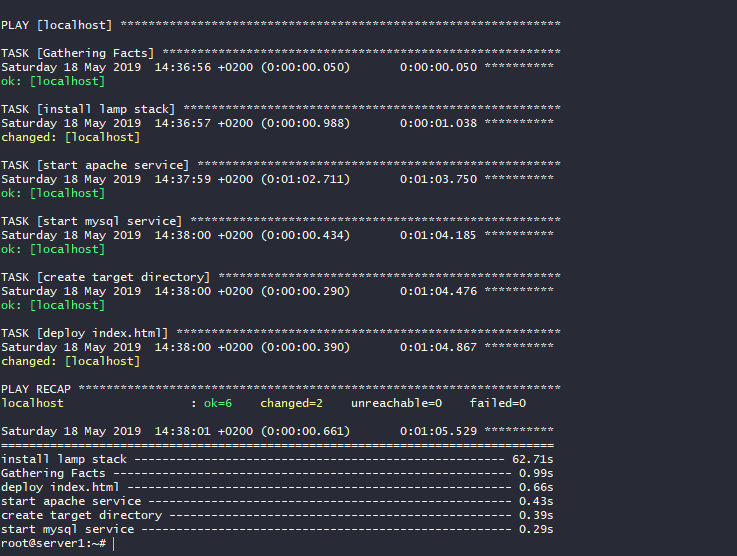
\includegraphics[width=0.45\textwidth]{img/ansibleoutput.png} }}%
    \caption{Cloud-init en Ansible outputs.}%
    \label{fig:outputs}%
\end{figure}

\section{Vergelijking met verwachte resultaten}
De verwachtingen zijn toch gedeeltelijke anders met de uiteindelijke resultaten/conclusies. In het voorstel werd er verwacht dat elke omgeving een ander oplossing ging hebben. Ook werd er verwacht dat de taken van Ansible en cloud-init gingen variëren van server tot server.

Dit is niet helemaal lijn met het effectieve resultaat. Er werd verwacht dat elke omgeving zijn eigen verhaal ging hebben en dat is toch niet gebeurt. Er kwam altijd één constante boven water. Cloud-init is goed voor de basis maar als er geavanceerder wilt gegaan worden is Ansible duidelijk beter. 

Uiteindelijk werd er verwacht dat cloud-init meer functionaliteiten ging hebben dan dat het uiteindelijk heeft. Er werd wel verwacht da Ansible ruimer ging zijn van mogelijkheden, aangezien dit veel populairder is. Maar er werd niet verwacht dat cloud-init er zoveel minder ging hebben.


\section{Verdere uitbreiding?}
Het onderzoek kan worden uitgebreid. Een restrictie die dit onderzoek had, is dat er maar met één cloud-provider kon worden gewerkt. Het zou interessant om te bekijken of er met andere providers hetzelfde resultaat zou hebben of niet. Ook de aanroeping van het cloud-init script en Ansible playbook kan op een andere manier. Door dit aan te aanroepen via een remote server. De servers worden dan opgesteld vanop een andere server en niet op de huidige server zoals hier. Weer zou het interessant zijn om te bekijken of een verandering invloed heeft op het resultaat.

De uiteindelijke vragen die na dit onderzoek kunnen worden gesteld zijn:
\begin{itemize}
    \item Hebben andere cloud-providers hetzelfde resultaat? 
    \item Heeft een andere aanroeping van de scripts een effect op het resultaat?
\end{itemize}



%%=============================================================================
%% Bijlagen
%%=============================================================================

\appendix

%%---------- Onderzoeksvoorstel -----------------------------------------------

\chapter{Onderzoeksvoorstel}

Het onderwerp van deze bachelorproef is gebaseerd op een onderzoeksvoorstel dat vooraf werd beoordeeld door de promotor. Dat voorstel is opgenomen in deze bijlage.

% Verwijzing naar het bestand met de inhoud van het onderzoeksvoorstel
%---------- Inleiding ---------------------------------------------------------

\section{Introductie} % The \section*{} command stops section numbering
\label{sec:introductie}

Voor de installatie van servers wordt al jaren Ansible gebruikt. Ansible is een universele 'taal' die taken voor servers automatiseert door middel van hun playbook. Zo een Ansible playbook is een georganiseerde unie van scripts dat het werk voor de server configuratie definieert.

Cloud-Init is momenteel een van de industrie standaarden voor het opbouwen van cloud servers, het maakt gebruik van cloud images. Dat zijn besturingssysteem sjablonen en elke instantie begint als een identieke kloon van elke andere instantie. De gebruikersgegevens geven elke cloud instantie haar persoonlijkheid. Doormiddel van cloud-int worden deze gegevens op de instantie toegepast. 

Dit zijn allebei provisioning systemen. Op een verschillende manier doen ze in theorie hetzelfde. Ze brengen de server allebei naar de gewenste toestand van de gebruiker. Doordat deze op verschillende manieren werken, wordt er in de praktijk in combinatie met beide gewerkt. In dat geval gebruik je eerste cloud-init om de server naar een gewenste toestand te brengen waar na Ansible het kan overnemen.

Maar is dit de perfecte samenwerking? Het bedrijf Be-mobile is opzoek naar het antwoord. In dit onderzoek bestuderen we waar deze mekaar aanvullen en hoe ze dan op een perfect performante manier werken. Natuurlijk is het goed mogelijk dat deze mekaar niet aanvullen en dan is het onderzoek waar en wanneer je voor wat moet kiezen en waarom dit mekaar overbodig maakt. 

In dit onderzoek zullen we dit trachten te ontdekken. De vragen waar het, de antwoorden op wil vinden zijn:
\begin{itemize}
	\item Vullen Ansible en Cloud-Init mekaar aan, of maken ze elkaar overbodig?
	\item Ook hoe ze mekaar aanvullen en/of hoe ze mekaar overbodig maken?
\end{itemize}

%Hier introduceer je werk. Je hoeft hier nog niet te technisch te gaan.

%Je beschrijft zeker:

%\begin{itemize}
%  \item de probleemstelling en context
%  \item de motivatie en relevantie voor het onderzoek
%  \item de doelstelling en onderzoeksvraag/-vragen
%\end{itemize}

%---------- Stand van zaken ---------------------------------------------------

\section{Stand Van Zaken}
\label{sec:state-of-the-art}

Ansible en Cloud-Init zijn geen onbekende voor mekaar dus er is wel een basis gevonden waarop er verder kan gewerkt worden. Maar zijn niet zo bekend dat de ultieme samenwerking al gevonden is. In het onderzoeken van de 2 systemen zijn er 5 artikels gevonden die een samenwerking beschrijven of afraden. 


In de artikels \textbf{"An introduction to server provisioning with CloudInit"\autocite{Cloudsigma}}, \textbf{“Using Ansible to Bootstrap My Work Environment Part 4” \autocite{scottharney}} en \textbf{“Customizing Cloud Assembly Deployments with Cloud-Init” \autocite{vmware}} is er een vaak voorkomend fenomeen gevonden. Meestal gebruiken de gebruikers/auteurs eerst cloud-init om de machine op te starten, daarna ansible voor de verdere specifieke eigenschappen.


Het artikel geschreven door \textcite{Cloudsigma} is wel interessant doordat hij ook andere systemen buiten cloud-init heeft getest, waaronder puppet en chef. Maar toch verkiest hij om Ansible te gebruiken. Dit betekent dat een samenwerking met ansible optimaler is.


De artikels \textbf{“Zero Touch Provisioning of Infoblox Grid on OpenStack using Ansible”\autocite{infoblox}} en \textbf{"Automated Ansible AWX Installation" \autocite{deven}} beschrijven dan weer hoe beide elke als een apart systeem kunnen worden gebruikt zonder de hulp van de ander. Maar toch zijn er een paar gelijkenissen zo gebruikt \textcite{deven} in "Automated Ansible AWX Installation" notities van een Ansible installatie om het met cloud-init te installeren.


Er is duidelijk al bekend dat er samengewerkt kan worden, maar ook soms weer niet. Maar criteria om te bepalen wanneer welke het best is, is nog niet bekend. 








%Hier beschrijf je de \emph{state-of-the-art} rondom je gekozen onderzoeksdomein. Dit kan bijvoorbeeld een literatuurstudie zijn. Je mag de titel van deze sectie ook aanpassen (literatuurstudie, stand van zaken, enz.). Zijn er al gelijkaardige onderzoeken gevoerd? Wat concluderen ze? Wat is het verschil met jouw onderzoek? Wat is de relevantie met jouw onderzoek?

%Verwijs bij elke introductie van een term of bewering over het domein naar de vakliteratuur, bijvoorbeeld~\autocite{Doll1954}! Denk zeker goed na welke werken je refereert en waarom.

% Voor literatuurverwijzingen zijn er twee belangrijke commando's:
% \autocite{KEY} => (Auteur, jaartal) Gebruik dit als de naam van de auteur
%   geen onderdeel is van de zin.
% \textcite{KEY} => Auteur (jaartal)  Gebruik dit als de auteursnaam wel een
%   functie heeft in de zin (bv. ``Uit onderzoek door Doll & Hill (1954) bleek
%   ...'')


%---------- Methodologie ------------------------------------------------------
\section{Methodologie}
\label{sec:methodologie}

Dit onderzoek zal gevoerd worden door virtuele server omgevingen op te zetten met Cloud-init en/of Ansible. De programma’s die hierbij zullen worden gebruikt zijn VirtualBox, Vagrant en Atom. 

Virtualbox is een programma om virtuele machines op te draaien. Met Vagrant kan je van in je shell met een simpel commando virtuele machines op starten. Atom is dan weer een teksteditor om de configuratie goed in neer te pennen. Normaal is deze het vermelden niet waar maar door de overzichtelijke manier van werken die het aanbiedt is deze toch veel beter dan een gewone Notepad.

Met Ansible zal er voor verschillende servers een testomgeving worden opgezet. Dit zal dan ook gebeuren met cloud-init. Deze resultaten en omgevingen kunnen dan worden  vergeleken met elkaar. De technische eigenschappen/resultaten worden dan onder de loep genomen: de performantie, de snelheid van het opstarten,… Ook zal er worden gekeken naar de config files van beiden en kan er worden gekeken welke daar per omgeving “beter” is. M.a.w. welke er op een kortere overzichtelijkere manier hetgeen kan bekomen. Be-Mobile kan ook nog verdere criteria bepalen waardoor we een keuze gaan maken. Daarna worden ook  combinaties van de twee aangemaakt en dan kunnen we deze vergelijken met de originele servers. 

Ook kan het zijn dat er vragen worden gesteld aan medewerkers van het bedrijf Be-Mobile om te bekijken wat hun mening over beide is.

%Hier beschrijf je hoe je van plan bent het onderzoek te voeren. Welke onderzoekstechniek ga je toepassen om elk van je onderzoeksvragen te beantwoorden? Gebruik je hiervoor experimenten, vragenlijsten, simulaties? Je beschrijft ook al welke tools je denkt hiervoor te gebruiken of te ontwikkelen.

%---------- Verwachte resultaten ----------------------------------------------
\section{Verwachte resultaten}
\label{sec:verwachte_resultaten}
De verwachtingen zijn dat een combinatie van cloud-init en Ansible meestal het beste zal zijn. Dat er voor elke server tot een bepaald moment cloud-init of ansible  zal worden gebruikt waarna ansible of cloud-init het zal overnemen. Ook zijn de verwachtingen dat er voor elke omgeving een andere oplossing zal zijn. Er zal veel afhangen van het type besturingssysteem dat draait en van de servers om te kunnen bepalen welke het best wordt gekozen. 

De verwachtingen zijn ook dat niet bij alles een combinatie zal worden gebruikt. Ook kan het misschien zijn dat het beter is dat je één van beide kiest voor een bepaalde server omgeving.


%Hier beschrijf je welke resultaten je verwacht. Als je metingen en simulaties uitvoert, kan je hier al mock-ups maken van de grafieken samen met de verwachte conclusies. Benoem zeker al je assen en de stukken van de grafiek die je gaat gebruiken. Dit zorgt ervoor dat je concreet weet hoe je je data gaat moeten structureren.

%---------- Verwachte conclusies ----------------------------------------------
\section{Verwachte conclusies}
\label{sec:verwachte_conclusies}
De verwachte conclusie is dat elke server omgeving een andere uitkomst zal hebben. Er veel zal afhangen van welke server je precies wilt draaien op welk systeem. Dan kan er worden gekozen voor een bepaalde combinatie van beide of misschien één van beide. De conclusie zal niet zijn welke van de twee beter is. Maar eerder hoe ze het best gebruikt worden per serveromgeving.



%Hier beschrijf je wat je verwacht uit je onderzoek, met de motivatie waarom. Het is \textbf{niet} erg indien uit je onderzoek andere resultaten en conclusies vloeien dan dat je hier beschrijft: het is dan juist interessant om te onderzoeken waarom jouw hypothesen niet overeenkomen met de resultaten.



%%---------- Andere bijlagen --------------------------------------------------
% TODO: Voeg hier eventuele andere bijlagen toe
%\input{...}

%%---------- Referentielijst --------------------------------------------------

\printbibliography[heading=bibintoc]
%\addcontentsline{toc}{chapter}{\textcolor{maincolor}{\IfLanguageName{dutch}{Bibliografie}{Bibliography}}}

\end{document}
